\section{Optical Spatial Modulation}
\label{sec:osm}

\graphicspath{{_MIMOSpace/figures_osm/}}

\subsection{Imaging SM and SMP System}
\label{subsec:osmSystem}
A simple optical MIMO system using an ImR for VLC applications is illustrated in \figurename{ \ref{figImagingSystem}}. Incoming data stream is coded and input to the modulator. The illumination state block provides a second input to the modulator which is the value of the average intensity to be emitted from each luminaire. Based on these inputs, the modulator block generates drive signals. $N_{tx}$ number of lumianires positioned on the ceiling act as optical transmitters while providing illumination. LEDs in the luminaire convert modulated data in the electrical domain into optical signals in the visible spectrum (E/O and conversely O/E conversion). These optical signals propagate through the indoor space and are incident on the receiver. The receiver performs O/E conversion. With apriori knowledge of the implemented modulation and coding schemes, the electrical signal is then demodulated and decoded to recover the transmitted information. \figurename{ \ref{figImagingReceiver}} illustrates a schematic of an ImR. The optical assembly consists of a filter, imaging lens, aperture and housing. $f$ is the focal length as set by the lens assembly. The sensor is made up of a matrix of $N_{px}$ contiguous pixels. The length of the shortest side of each pixel is $\alpha_{px}^{min}$ and the pixel diagonal is $\alpha_{px}^{max}$. The sensor is assumed to always be located distance $f$ away from the optical center of the lens.

\begin{figure}[!b]
	\centering
		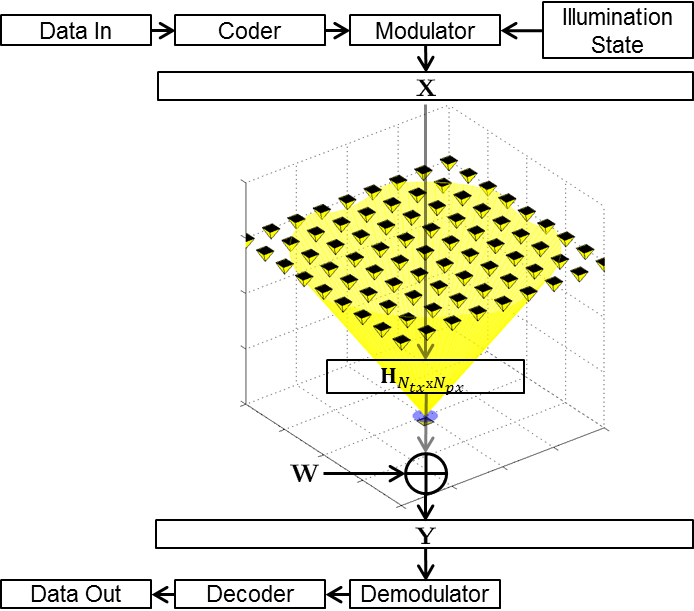
\includegraphics[width=5in]{figImagingSystem.png}
	\caption{Schematic of an optical MIMO system.}
	\label{figImagingSystem}
\end{figure}
%\begin{figure}[!t]
	%\centering
		%\includegraphics[width=3in]{_figureSetup.eps}
	%\caption{Schematic of an optical MIMO system.}
	%\label{figImagingSystem}
%\end{figure}

The imaging optics acts as an optical demultiplexer. Based on the angle and the location of incidence, light rays are redirected by the imaging optics on to a specific path. This helps to decorrelate the channel matrix coefficients. Similarly, the ambient radiant flux incident at the aperture of the receiver is distributed among all pixels of the sensor. This helps to significantly reduce shot noise per pixel \cite{dja00a}. The channel can then be modeled as
\begin{equation}
	\label{eqMimoChannel}
	\bf{Y} = \bf{H}\bf{X} + \bf{W}
\end{equation}
where {\bf{X}} is the intensity modulated input signal vector of length $N_{tx}$. The channel matrix {\bf{H}} takes into account the path-loss, transmission of the optics and the responsivity of the sensor pixels. It can be computed as in reference \cite{but13a}. {\bf{Y}} is the $N_{px}$ length output current vector. ${\bf{W}}\sim\mathcal{N}({\bf{0}},\sigma^2{\bf{I}}_{N_{px}})$ is the additive white Gaussian noise (AWGN) vector.

\begin{figure}[!t]
	\centering
		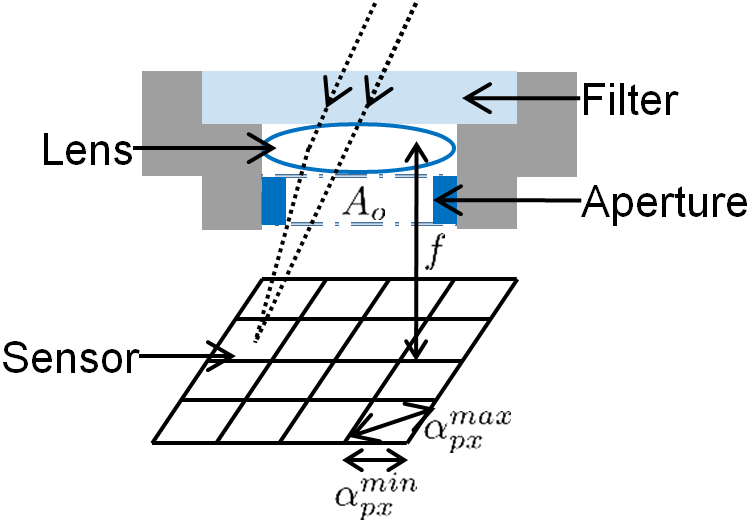
\includegraphics[width=3in]{figImagingReceiver.png}
	\caption{Schematic of an imaging receiver.}
	\label{figImagingReceiver}
\end{figure}

\begin{figure}[!b]
	\centering
		\begin{subfigure}{0.49\textwidth}
		\centering
				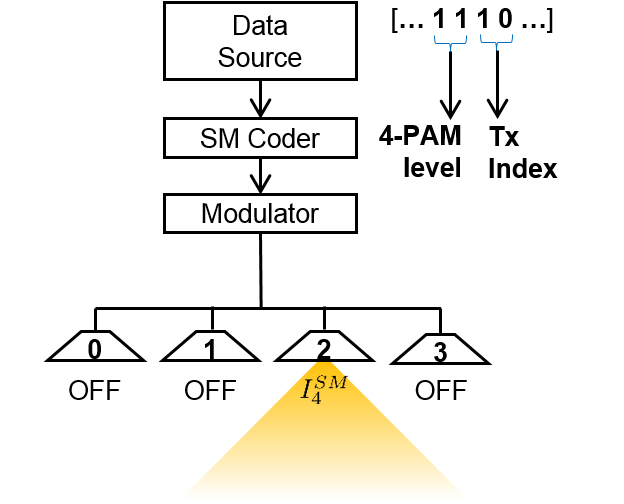
\includegraphics[trim=0in 0in 0in 0in, clip=false, width=2.5in]{figSM.png}
		\caption{}
		\label{figSM}			
		\end{subfigure}
		\hfill
		\begin{subfigure}{0.49\textwidth}
		\centering
				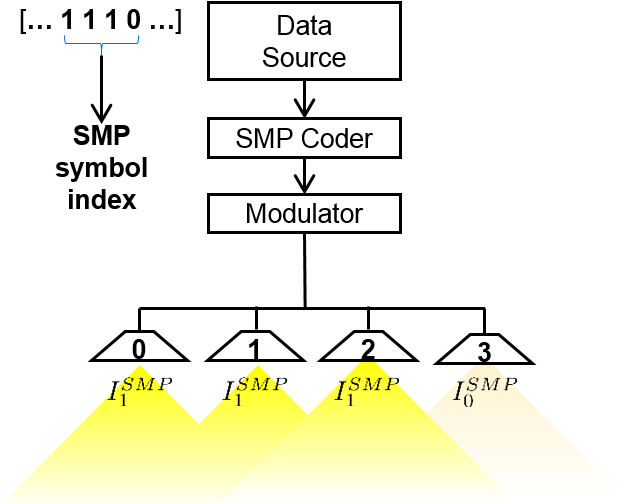
\includegraphics[trim=0in 0in 0in 0in, clip=false, width=2.5in]{figSMP.png}
				\caption{}
				\label{figSMP}
		\end{subfigure}
\caption{Illustration of (a) SM operation with $N_{tx} = 4$ and $M = 4$. (b) SMP operation with $N_{tx} = 4$ and $M = 2$.}
	\label{fig:SpatialModulation}
\end{figure}

SM encodes $k=log_2(N_{tx})$ bits in the transmitter index in addition to $m=log_2(M)$ bits using M-ary modulation. Thus SM achieves spectral efficiency of $r=k+m=log_2(MN_{tx})$ bits/s/Hz. The incoming data stream is divided into $r$ bits long symbols. First $m$ bits of each symbol are mapped to one of the M-ary constellation points while the last $k$ bits of each symbol select the luminaire that transmits the selected constellation point. SM implementation is illustrated in \figurename{ \ref{figSM}} for $N_{tx}=4$ transmitters and 4-PAM (pulse amplitude modulation). M-PAM intensity levels for SM are selected as in (\ref{eqSMPAM}) where $I_{avg}$ is the average signal constraint to maintain desired illumination. Given a bit sequence forming a symbol [1 1 1 0], PAM level 3 $(I_4^{SM})$ is sent on transmitter index $2$.

\begin{equation}
	\label{eqSMPAM}
	I_{x}^{SM} = \frac{2I_{avg}}{M+1}x; x=1\hdots M
\end{equation}

On the other hand, SMP uses all luminaires to jointly transmit information. If each of the $N_{tx}$ luminaires can transmit M-ary modulation such that they jointly generate $M^{N_{tx}}$ unique symbols, spectral efficiency of SMP is given by $r=N_{tx}log_2(M)$ bits/s/Hz. Each $r$ bit long section of the incoming data stream is then mapped to one of the $M^{N_{tx}}$ unique symbols. SMP for a setup with $N_{tx}=4$ transmitters and 2-PAM is illustrated in \figurename{ \ref{figSMP}}. M-PAM intensity levels for SMP are selected as in (\ref{eqSMPPAM}) where $I_{avg}$ is the average signal constraint to maintain desired illumination. A bit sequence forming a symbol [1 1 1 0] is jointly mapped to the $15^{th}$ out of $N_{tx}log_2(M)=16$ possible unique symbols.
\begin{equation}
	\label{eqSMPPAM}
	I_{x}^{SMP} = \frac{2I_{avg}}{M-1}x; x=0\hdots M-1
\end{equation}

For a channel with equally likely symbols, a maximum likelihood detector is the optimal detector. If noise is AWGN, this reduces to nearest neighbor detection. Having observed ${\bf{Y}}$ and knowing ${\bf{H}}$, estimated symbol $\hat{{\bf{X}}}$ is the symbol closest to observation ${\bf{Y}}$ in Euclidean space. The signal detection can be written as
\begin{gather}
\begin{aligned}
	\hat{{\bf{X}}} =&{} \argmax_{{\bf{X_i}}} p_{{\bf{Y}}|{\bf{X}}}({\bf{Y}}|{\bf{X_i}},{\bf{H}})\\
	=&{} \argmin_{{\bf{X_i}}} ||{\bf{Y}}-{\bf{H}}{\bf{X_i}}||_{F}
\label{eq:ML}
\end{aligned}
\end{gather}
where ${\bf{X_i}}$ are the different symbols and $||.||_{F}$ is the Frobenius norm.

%%%%%%%%%%%%%%%%%%%%%%%%%%%%%%%%%%%%%%%%%%%%%%%%%%%%%%%%%%%%%%%%
%%%%%%%%%%%%%%%%%%%%%%%%%%%% OSM IMG %%%%%%%%%%%%%%%%%%%%%%%%%%%
%%%%%%%%%%%%%%%%%%%%%%%%%%%%%%%%%%%%%%%%%%%%%%%%%%%%%%%%%%%%%%%%

\subsection{Imaging Spatial Modulation and Multiplexing}
\label{subsec:osmImaging}
MIMO indoor optical systems implementing an imaging receiver have been
shown to greatly increase the capacity of the channel over a SISO
system operating under similar power constraints
\cite{but13a}. \figurename{\ref{fig:ImagingSystem}} illustrates a
simple optical MIMO system using an imaging receiver. Lumianires
positioned on the ceiling act as optical transmitters while providing
illumination. LEDs in the luminaire convert modulated data in the
electrical domain into optical signals within the visible
spectrum. These optical signals propagate through the indoor space and
are captured by a sensor that performs optical to electrical
conversion. The electrical signals are used to recover the data.

\begin{figure}
	\centering
		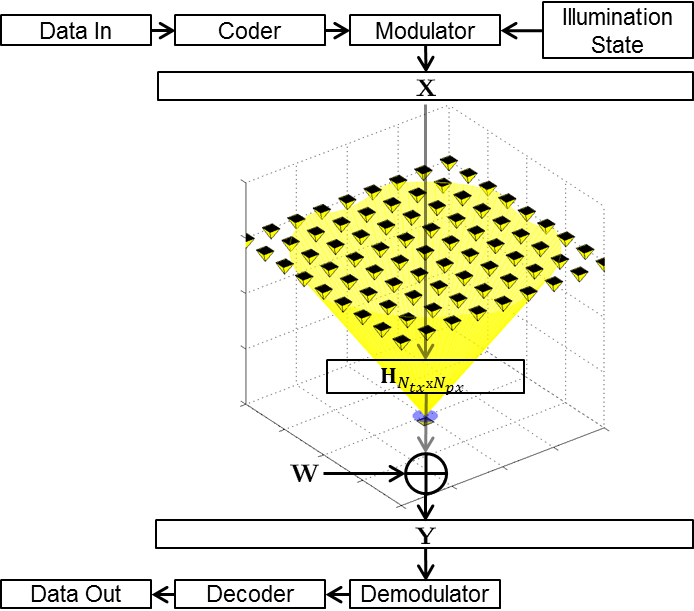
\includegraphics[width=2.5in]{figImagingSystem.png}
	\caption{Optical MIMO System with Imaging Receiver}
	\label{fig:ImagingSystem}
\end{figure}

Imaging receivers for optical communication have been proposed in \cite{kah98a}. The imaging optics act like an optical demultiplexer. Based on angle and location of incidence, light rays are redirected by imaging optics on to a specific path. This helps decorrelate channel matrix coefficients. This same phenomenon distributes the ambient radiant flux incident at the aperture of the receiver among all pixels of the sensor. This helps significantly reduce shot noise per pixel \cite{dja00a}.

\figurename{\ref{fig:ImagingReceiver}} illustrates a schematic of an imaging receiver. This is made up of an optical assembly and a sensor. The optical assembly consists of an optical filter, a lens assembly, an aperture and a housing to carry the parts. $A_{o}$ is the area of the aperture opening. The lens assembly may consist of one or more lenses to minimize distortions. $f$ is the focal length as set by the lens assembly. The sensor is made up of a matrix of contiguous pixels. The length of the shortest side of each pixel is $\alpha_{px}^{min}$. It is assumed that there is some form of an on-chip bus architecture that routes the received signals to a receiving computer that performs the signal processing.

\begin{figure}
	\centering
		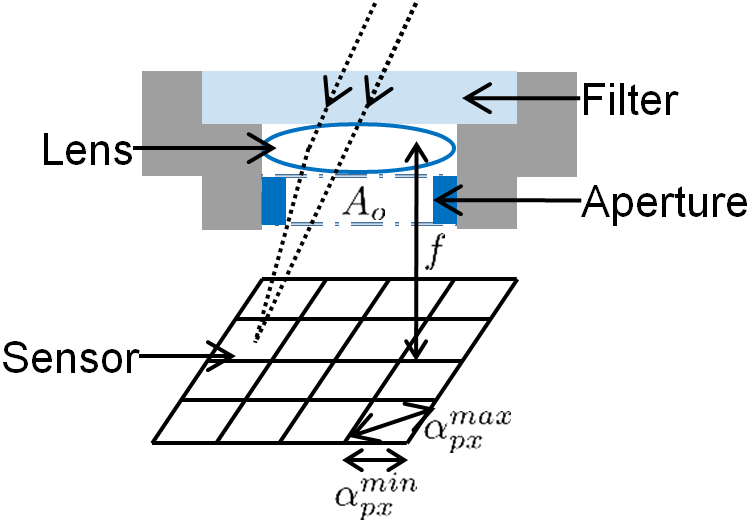
\includegraphics[width=3in]{figImagingReceiver.png}
	\caption{Schematic of Imaging Receiver}
	\label{fig:ImagingReceiver}
\end{figure}

A MIMO indoor optical channel with imaging receiver can be modeled as (\ref{eqMimoChannel2}). {\bf{X}} is the intensity modulated input signal vector of length $N_{tx}$. {\bf{Y}} is an $N_{px}$ length vector containing output currents. {\bf{H}} is the channel matrix taking into account the losses due to free space propagation, optical losses and channel decorrelation at the imaging optics and the responsivity of the receiver photodiodes. ${\bf{W}}\sim\mathcal{N}({\bf{0}},\sigma^2{\bf{I_{px}}})$ is the AWGN vector. Thermal noise is assumed the dominant source of noise \cite{dja00a}. The $N_{px}$x$N_{tx}$ channel matrix ${\bf{H}}$ is computed as in \cite{but13a}.

%Multiple ($N_{tx}$) transmitters are positioned on the ceiling in a regular grid. The length of the longest segment across the transmitter illumination surface is given by $\alpha_{tx}^{max}$. 

\begin{equation}
	\label{eqMimoChannel2}
	\bf{Y} = \bf{H}\bf{X} + \bf{W}
\end{equation}

For a channel with equally likely symbols, ML detector is the optimal detector. If noise is AWGN, this reduces to NN detection. Having observed ${\bf{Y}}$ and knowing ${\bf{H}}$, estimated symbol $\hat{{\bf{X}}}$ is the symbol closest to observation ${\bf{Y}}$ in Euclidean space.

%\setlength{\arraycolsep}{0.0em}
\begin{gather}
\begin{aligned}
	\hat{{\bf{X}}} =&{} \argmax_{{\bf{X_i}}} p_{{\bf{Y}}|{\bf{X}}}({\bf{Y}}|{\bf{X_i}},{\bf{H}})\\
	=&{} \argmin_{{\bf{X_i}}} ||{\bf{Y}}-{\bf{H}}{\bf{X_i}}||_{F}
\label{eq:ML2}
\end{aligned}
\end{gather}
%\setlength{\arraycolsep}{5pt}

It is desired to analyze the effect of receiver configuration on performance of spatial multiplexing (SMux) and spatial modulation (SMod). An example system is considered which has 4 transmitters arranged on a regular grid with pitch $P_{tx}$. Each transmitter has side length $\alpha_{tx}^{min}$ and diagonal $\alpha_{tx}^{max}$. The imaging receiver optics has focal length $f$. Sensor is made of large enough contiguous PD array such that all the 4 transmitter images (spots) fall on the sensor for all the different analysis configurations. Each PD is assumed to have a square shape with side length $\alpha_{px}^{min}$ and diagonal $\alpha_{px}^{max}$. The receiver surface is assumed parallel to the transmitter plane. Receiver at a distance $d$ from the transmitter plane sees a magnification $M=f/(d-f)$. If $d>>f$, which is true is most practical scenarios, $M\approx f/d$. The system performance is dependent on how the spots land on the PD array. Different system configurations can generate similar spot profile on the sensor and thus similar BER performance.  To analyze the system performance independent of a specific system configuration, the following normalization parameters are defined.

\subsubsection{Normalized Luminaire Side Length}
\label{subsubsec:osmImagingSide}
The normalized luminaire side length $\alpha_{s}$ is defined as the ratio of the diagonal of a spot to side length of a PD. 
\begin{equation}
	\label{eqAlphaS}
	\alpha_{s} \equiv \frac{M a_{tx}^{max}}{\alpha_{px}^{min}}
\end{equation}
$\alpha_{s}$ specifies the spot size relative to the sensor dimensions. For example, consider two similar systems which differ in only the luminaire diagonal and PD side lengths. If both parameters differ in scale by the same factor, $\alpha_{s}$ would remain the same for both systems. $\alpha_{s}\leq 1$ implies the spot size is at most as large as the size of a PD. If the centroid of the spot is aligned with the centroid of a PD, the spot will lie completely inside the PD.
 
\subsubsection{Normalized Luminaire Pitch}
\label{subsubsec:osmImagingPitch}
The normalized luminaire pitch $\delta_{s}$ is defined as the ratio of the spot pitch to the length PD diagonal. 
\begin{equation}
	\label{eqDeltaS}
	\delta_{s} \equiv \frac{M P_{tx}}{\alpha_{px}^{max}}
\end{equation}
$\delta_{s}$ specifies the distance between the centroids of adjacent spots relative to the sensor dimensions. For example, now consider two similar systems which differ in only the transmitter pitch and PD diagonal. If both parameters differ in scale by the same factor, $\delta_{s}$ would remain the same. $\delta_{s}>1$ ensures that centroids of adjacent spots lie on different pixels. In the limit, if both transmitters were point sources, condition $\delta_{s}>1$ would ensure that different pixels receive signals from neighboring transmitters, thus eliminating ICI.

\subsubsection{Normalized Luminaire Edge-Edge Distance}
\label{subsubsec:osmImagingEdge}
The normalized luminaire edge-edge distance $\eta_{s}$ is defined as the ratio of minimum distance between the edges of adjacent spots to the length of the pixel diagonal.
\begin{equation}
	\label{eqEtaS}
	\eta_{s} \equiv \frac{M(P_{tx}-\alpha_{tx}^{max})}{\alpha_{px}^{max}}
\end{equation}
$\eta_{s}$ specifies the minimum possible distance between the edges of adjacent spots relative to the sensor dimensions. For example, now consider two similar systems which differ in only the minimum possible distance between the edges of adjacent luminaires and PD diagonal. If both parameters scaled by the same factor, $\eta_{s}$ would remain the same. $\eta_{s}>1$ ensures that adjacent spots do not overlap on any pixel. $\eta_{s}$ can be expressed in terms of $\alpha_{s}$ and $\delta_{s}$ as in (\ref{eqES2}). For square pixels, $l=1/\sqrt{2}$.

\begin{eqnarray}
	l &= \frac{\alpha_{px}^{min}}{\alpha_{px}^{max}}\label{eqESl}\\
	\eta_{s} &= \delta_{s} - l\alpha_{s}\label{eqES2}
\end{eqnarray}

\subsubsection{Normalized Magnification}
\label{subsubsec:osmImagingMagnification}
Let $M_0$ be the magnification of the system when $\alpha_{s}=1$. Normalized magnification is defined as the ratio of the magnification of the system to $M_0$.

\begin{eqnarray}
	M_{0} &\equiv \frac{\alpha_{rx}^{min}}{\alpha_{tx}^{max}}\label{eqM0}\\
	\mu_{s} &\equiv \frac{M}{M_{0}}\label{eqMS}
\end{eqnarray}

Consider two similar systems that differ in distance between the luminaire plane and the receiver and also in the receiver focal lengths. $\mu_{s}$ for both systems is the same value when both parameters differ in scale by the same factor.

In an indoor VLC system, luminaires need to maintain an average emitted radiant flux over different overlapping time windows so that the perceived illumination remains constant. Thus a fair performance comparison between different modulation schemes can be made when they emit the same radiant flux. Thus the SNR is defined as
\begin{equation}
	SNR = \frac{(hP_{avg}^{tx})^2}{\sigma^2}
\end{equation}
where $P_{avg}^{tx}$ is the average radiant flux emitted by a transmitter, $h$ is the optical to electrical conversion factor $(AW^{-1}\Omega^{-2})$ and $\sigma^2$ is the noise power. Without loss of generality, $h=1$ is assumed. This is similar definition as in \cite{fat13a}

%%%%%%%%%%%%%%%%%%%%%%%%%%%%%%%%%%%%%%%%%%%%%%%%%%%%%%%%%%%%%%%%
%%%%%%%%%%%%%%%%%%%%%%%%%%%% RESULTS %%%%%%%%%%%%%%%%%%%%%%%%%%%
%%%%%%%%%%%%%%%%%%%%%%%%%%%%%%%%%%%%%%%%%%%%%%%%%%%%%%%%%%%%%%%%

\subsection{Results}
\label{subsec:osmResults}
The effects of varying transmitter array and ImR configurations on the BER performance of SM and SMP systems are studied using simulations. An array of 4 transmitters that are arranged on a regular grid with pitch $P_{tx}$ is considered. Using PAM, and to achieve 4 bits/sym, SM with $N_{t}=4$ and $M=4$ and SMP with $N_{t}=4$ and $M=2$ are implemented. To achieve 8 bits/sym, SM with $N_{t}=4$ and $M=64$ and SMP with $N_{t}=4$ and $M=4$ are implemented. The distance $d$ between the transmitter and receiver planes is 2$m$. Lambertian luminaires of order $m=1$ are assumed to have a spectral power distribution that is approximated by a sum of gaussians as in \cite{gru08b}. The responsivity of each pixel is equal to $0.4A/W$. Within this context, it is assumed that the pixels array is large enough to ensure that each of the four spots fall on the sensor for each of the different configurations considered below.

Using the parameters specified above, the channel gains are of the order of $10^{-7}$ for all simulations. Thus the transmitted signal power is about $140$dB higher than the received signal power. Typically, the SNR is defined as the ratio of received signal power to noise power. However, given SNR as defined in {\color{red}(XYZ)}, there is an offset of at least $+140$dB over typical definition.

%%%%%%%%%%%%%%%%%%%%%%%%%%%%%%%%%%%%%%%%%%%
%%%%%%%%%%%%%%%%% COMPARE %%%%%%%%%%%%%%%%%
%%%%%%%%%%%%%%%%%%%%%%%%%%%%%%%%%%%%%%%%%%%
\subsubsection{Imaging vs Non-Imaging Receiver}
\label{subsubsec:osmResultsCompare}
Performance gains of using an ImR over a NImR are analyzed in this subsection. The transmitter and modulation parameters are the same as described above. For this analysis, $P_{tx}=0.5m$ is considered. The NImR is made up of $2\times2$ array of pixels; each with a side length of 1 mm and a pitch of 1 mm. Each pixel has a concentrator of refractive index $1.5$ and field-of-view (FOV) of $60\deg$. For the ImR, the sensor is modeled as $2\times2$ array of pixels with side length and pitch of $1mm$. The imaging lens is defined to have sufficient magnification to align the images of the four transmitters each with four pixels respectively. 
\begin{figure}[!b]
	\centering
		\begin{subfigure}{\textwidth}
			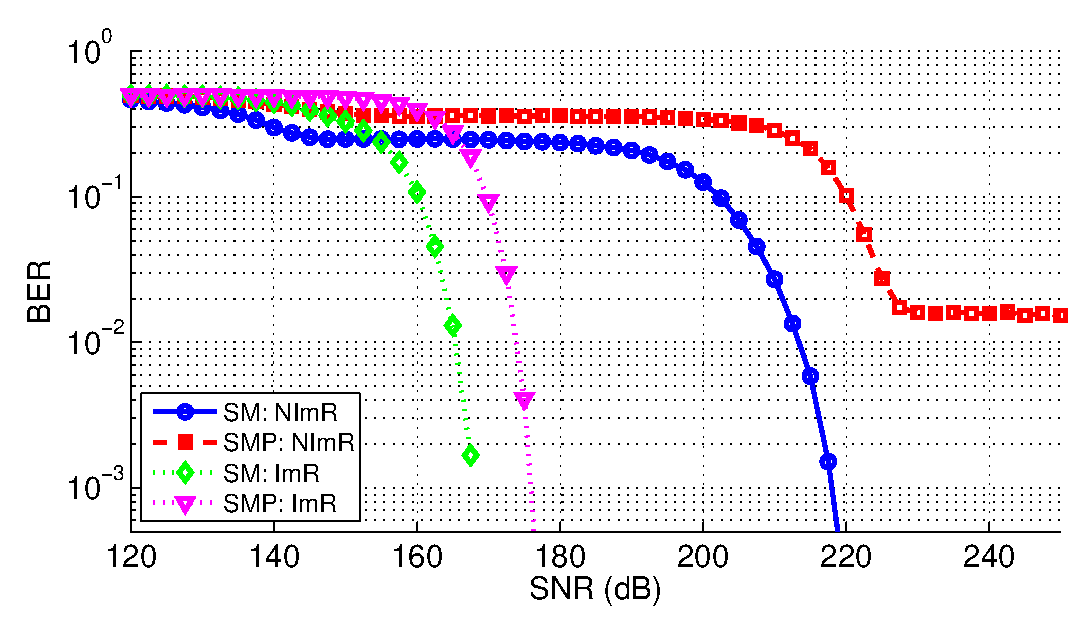
\includegraphics[width=\textwidth]{figCompare4B.eps}
			\caption{4 bits/sym}
			\label{figCompare4B}
		\end{subfigure}
	
		\begin{subfigure}{\textwidth}
		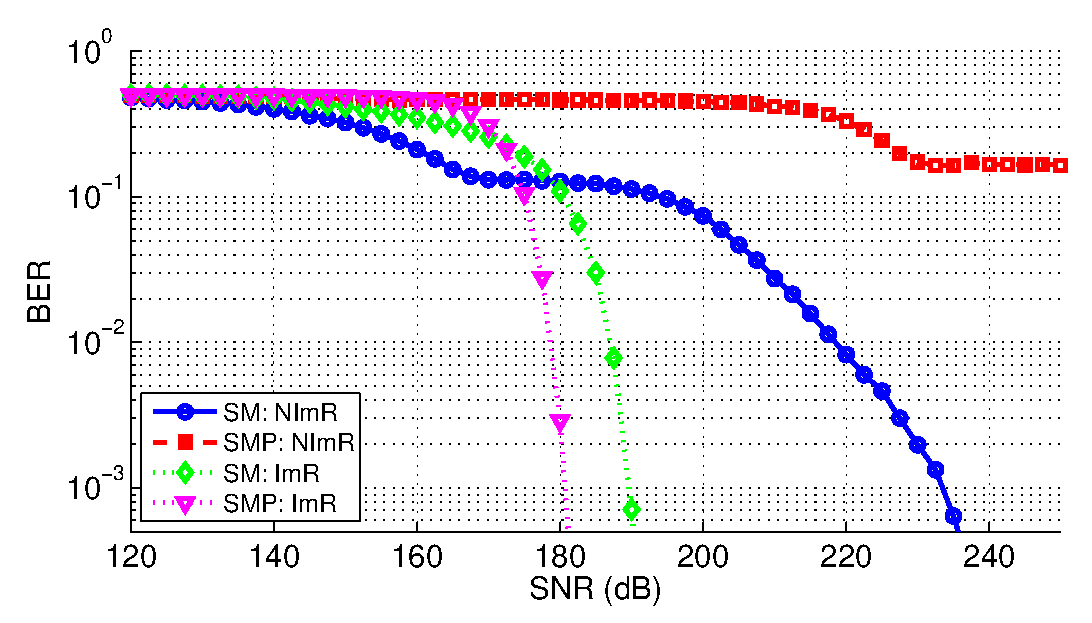
\includegraphics[width=\textwidth]{figCompare8B.eps}
		\caption{8 bits/sym}
		\label{figCompare8B}
		\end{subfigure}
	
	\caption{Performance comparison of SM and SMP using non--imaging an imaging receiver.}
	\label{figCompare}
\end{figure}
The FOV of the receiver changes with the sensor dimensions. The maximum FOV is defined as $60\deg$; the same as in NImR case. A fair performance comparison between the two receiver configurations can be made under the assumption that the same signal radiant-flux is incident on both. Thus, the aperture of the ImR is modeled to have an area of $1mm^{2}$.

BER vs SNR curves for SM and SMP using NImR and ImR are shown in \figurename{ \ref{figCompare}}. At low signal powers, using a NImR, shot noise is the dominant source of noise. At high signal powers, inter-channel-interference (ICI) dominates the noise for an NImR because the channel matrix coefficients are highly correlated. This can be seen as two regions of the BER curves when using a NImR. SM mitigates ICI and is thus more robust as compared to SMP in this scenario. BER achieved by SMP with NImR are greater than $10^{-3}$ for the range of SNR considered and thus cannot be improved by forward error correction (FEC). SM needs a high transmit signal power to achieve BER$=10^{-3}$ for both 4 and 8 bits/sym. Conversely, ImR completely demultiplexes the four transmit signals while generating a diagonal channel matrix and thus avoids ICI under ideal setup. To achieve BER$=10^{-3}$ at 4 bits/sym, SM with ImR performs about 8dB better that SMP with ImR and about 45dB better than SM with NImR. SMP packs more bits spatially in transmitter location as compared to SM. Thus, to achieve higher spectral efficiency while keeping the number of transmitters the same, more PAM levels are needed for SM as compared to SMP thus quickly degrading SM's performance. To achieve BER$=10^{-3}$ at 8 bits/sym, SMP with ImR outperforms SM with ImR by about 10dB and SM with NImR by about 52dB. The channel matrix coefficient decorrelation afforded by ImR provide huge SNR gains over NImR for a given BER.

\newpage
%%%%%%%%%%%%%%%%%%%%%%%%%%%%%%%%%%%%%%%%%%%%
%%%%%%%%%%%%%%%%%%% ALPHA %%%%%%%%%%%%%%%%%%
%%%%%%%%%%%%%%%%%%%%%%%%%%%%%%%%%%%%%%%%%%%%

\subsubsection{Varying $\alpha_{s}$}
\label{subsec:osmResultsAlpha}
For this analysis, $\alpha_{s}$ is varied while keeping $\delta_{s}$ and $\mu_{s}$ fixed. As illustrated in \figurename{ \ref{figASSpots}}, $\alpha_{s}$ affects only the spot size. As $\alpha_{s}$ increases, spots on the sensor overlap increasingly more number of pixels degrading the BER performance. Increasing the number or pixels per spot also increases the noise for each link thus causing the drop in performance. Very small pixel sizes or very large transmitter sizes also cause increase in $\alpha_{s}$. A smaller pixel size does enable the system to pack more channels provided $\alpha_{s}$ is relatively small. On the other hand, having very small pixel sizes or alternately large transmitter illumination surface tend to increase $\alpha_{s}$ and force the system to operate in a suboptimal configuration.

BER vs SNR curves for SM and SMP for different values of $\alpha_{s}$ are shown in \figurename{ \ref{figASBvS}}. To achieve BER$\leq10^{-3}$ at 4 bits/sym, SNRs of about [168,168,170,173]dB and [176,176,178,181]dB are needed for $\alpha_{s}$=[0.5,1,1.41,2]  with SM and SMP respectively. To achieve BER$\leq10^{-3}$ at 8 bits/sym, SNRs of about [190,190,192,195]dB and [181,181,183,186]dB are needed for $\alpha_{s}$=[0.5,1,1.41,2] with SM and SMP respectively. Thus there is about a 2dB SNR penalty for system operating at $\alpha_{s}=1.41$ and 5dB SNR penalty for system operating at $\alpha_{s}=2$ as compared to that at $\alpha_{s}=1$.

\begin{figure}[!b]
	\centering
		\begin{subfigure}{0.49\textwidth}
			\centering
			\includegraphics[width=1.5in]{figASspN4A05.eps}
			\label{figASspN4A05}
		\caption{$\alpha_{s}=0.5$}
		\end{subfigure}
		\hfill
		\begin{subfigure}{0.49\textwidth}
			\centering
			\includegraphics[width=1.5in]{figASspN4A1.eps}
			\label{figASspN4A1}
		\caption{$\alpha_{s}=1.0$}
		\end{subfigure}
		\vfill
		\begin{subfigure}{0.49\textwidth}
			\centering
			\includegraphics[width=1.5in]{figASspN4A14.eps}
			\label{figASspN4A14}
		\caption{$\alpha_{s}=1.41$}
		\end{subfigure}
		\hfill
		\begin{subfigure}{0.49\textwidth}
			\centering
			\includegraphics[width=1.5in]{figASspN4A2.eps}
			\label{figASspN4A2}
		\caption{$\alpha_{s}=2.0$}
		\end{subfigure}
		
	\caption{Spots on the sensor for different $\alpha_{s}$}
	\label{figASSpots}
\end{figure}

\begin{figure}
	\centering
		\begin{subfigure}{\textwidth}
			\centering
			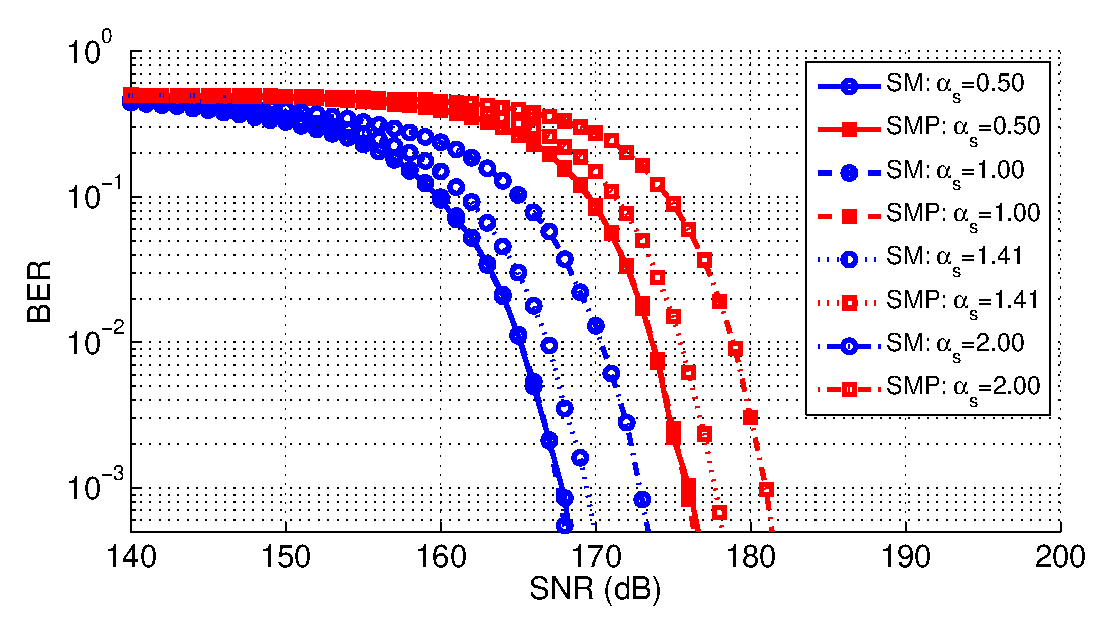
\includegraphics[width=\textwidth]{figASN4B4.eps}
			\caption{4 bits/sym}
			\label{figASN4B4}
		\end{subfigure}
		
		\begin{subfigure}{\textwidth}
			\centering
			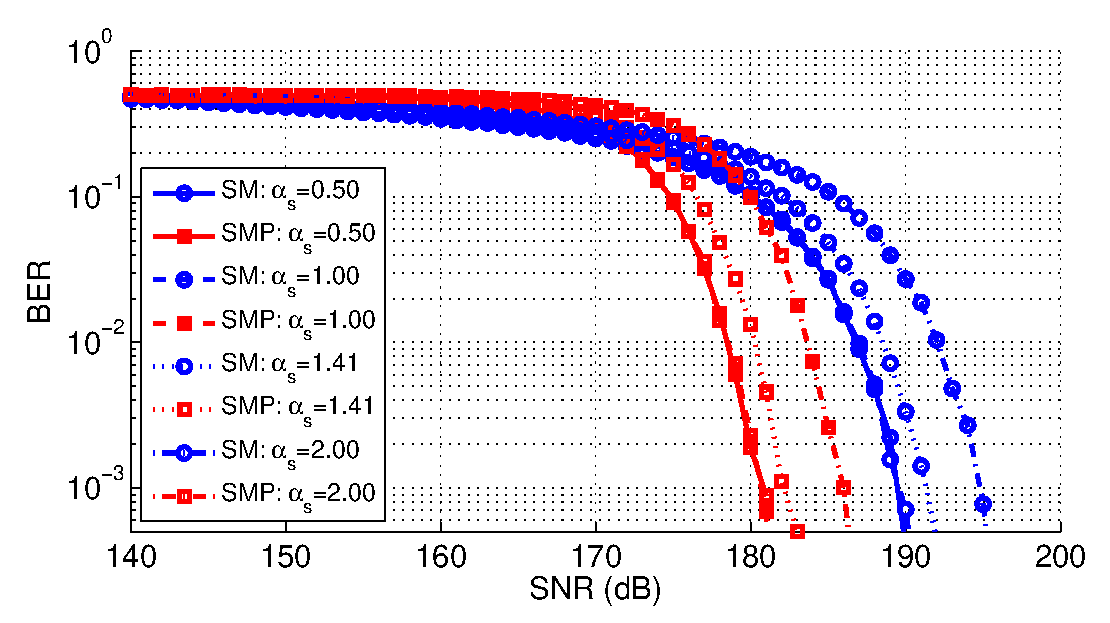
\includegraphics[width=\textwidth]{figASN4B8.eps}
			\caption{8 bits/sym}
			\label{figASN4B8}
		\end{subfigure}
		
		\caption{BER vs SNR for different $\alpha_{s}$.}
		\label{figASBvS}
\end{figure}

\newpage
%%%%%%%%%%%%%%%%%%%%%%%%%%%%%%%%%%%%%%%%%%
%%%%%%%%%%%%%%%%%%% ETA %%%%%%%%%%%%%%%%%%
%%%%%%%%%%%%%%%%%%%%%%%%%%%%%%%%%%%%%%%%%%
\subsubsection{Varying $\eta_{s}$}
\label{subsubsec:osmResultsEta}

For this analysis, $\eta_{s}$ (alternately $\delta_{s}$) is varied while keeping $\alpha_{s}$ and $\mu_{s}$ fixed. Thus only the effect of change in spot pitch affects the BER performance. As illustrated in \figurename{ \ref{figESSpots}}, as $\eta_{s}$ increases, distance between the spots on the sensor increases as they push further apart.

BER vs SNR curves for SM and SMP for different values of $\eta_{s}$ are shown in \figurename{ \ref{figESBvS}}. To achieve BER$\leq 10^{-3}$ at 4 bits/sym, SNRs of about [167,174,172,170]dB and [175,182,180,178]dB are needed for $\eta_{s}$=[0,0.71,1,1.41] with SM and SMP respectively. To achieve BER$\leq 10^{-3}$ at 8 bits/sym, SNRs of about [189,196,194,192]dB and [180,187,185,183]dB are needed for $\eta_{s}$=[0,0.71,1,1.41] with SM and SMP respectively. We see that the BER performance is best when the spot overlaps minimum number of pixels and worst when the spot is centered at a corner of a pixel thus maximizing the number of pixels it overlaps with. In this setup, for BER$=10^{-3}$, there is an SNR penalty of about 7dB between the best and worst cases. The slight drop in performance for $\eta_{s}=1.4$ as compared to $\eta_{s}=0$ can be attributed to drop in free-space gain caused by the larger distance per link longer as a result of increased transmitter pitch.

\begin{figure}
	\centering
		\begin{subfigure}{0.49\textwidth}
			\centering
			\includegraphics[width=1.5in]{figESspN4E0.eps}
			\caption{$\eta_{s}=0$}
			\label{figESspN4E0}
		\end{subfigure}
		\hfill
		\begin{subfigure}{0.49\textwidth}
			\centering
			\includegraphics[width=1.5in]{figESspN4E071.eps}
			\caption{$\eta_{s}=0.71$}
			\label{figESspN4E071}
		\end{subfigure}
		\vfill
		\begin{subfigure}{0.49\textwidth}
			\centering
			\includegraphics[width=1.5in]{figESspN4E1.eps}
			\caption{$\eta_{s}=1$}
			\label{figESspN4E1}
		\end{subfigure}
		\hfill
		\begin{subfigure}{0.49\textwidth}
			\centering
			\includegraphics[width=1.5in]{figESspN4E14.eps}
			\caption{$\eta_{s}=1.41$}
			\label{figESspN4E14}
		\end{subfigure}
		
		\caption{Spots on sensor for different $\eta_{s}$}
		\label{figESSpots}
\end{figure}

\begin{figure}
	\centering
		\begin{subfigure}{\textwidth}
			\centering
			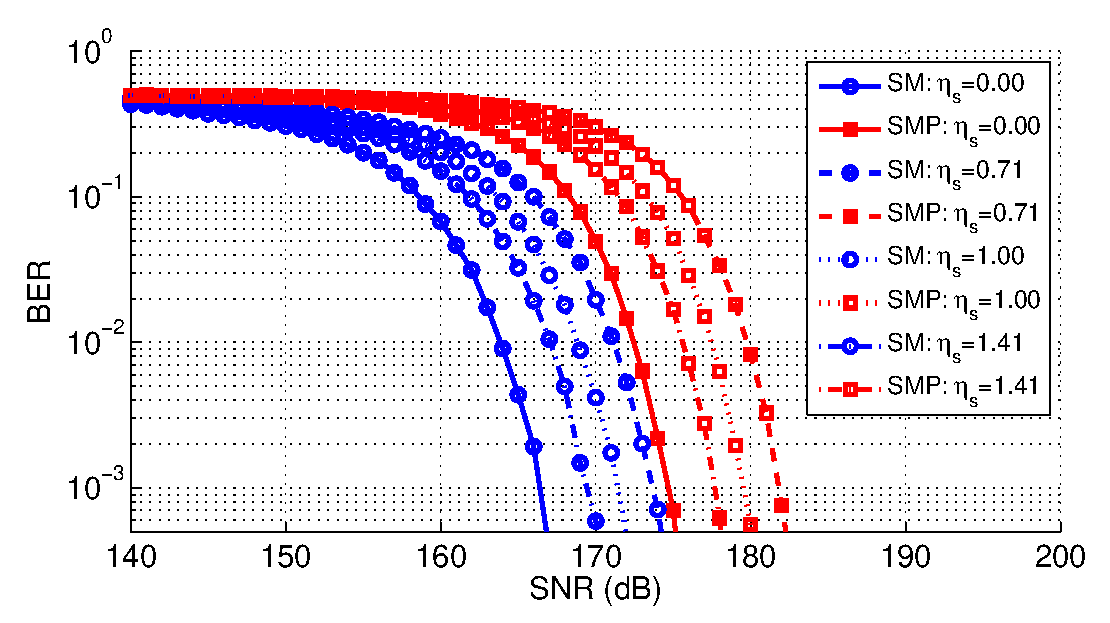
\includegraphics[width=\textwidth]{figESN4B4.eps}
			\caption{4 bits/sym}
			\label{figESN4B4}
		\end{subfigure}
		
		\begin{subfigure}{\textwidth}
			\centering
			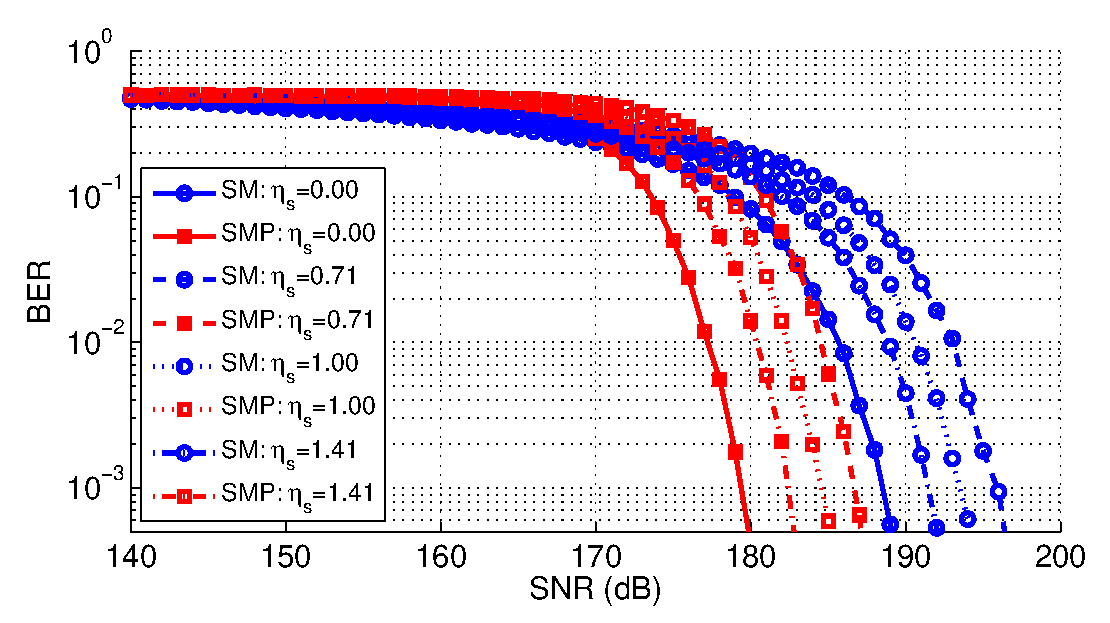
\includegraphics[width=\textwidth]{figESN4B8.eps}
			\caption{8 bits/sym}
			\label{figESN4B8}
		\end{subfigure}
		
		\caption{BER vs SNR for different $\eta_{s}$.}
		\label{figESBvS}
\end{figure}
\newpage
%%%%%%%%%%%%%%%%%%%%%%%%%%%%%%%%%%%%%%%%
%%%%%%%%%%%%%%%%%% MU %%%%%%%%%%%%%%%%%%
%%%%%%%%%%%%%%%%%%%%%%%%%%%%%%%%%%%%%%%%
\subsubsection{Varying $\mu_{s}$}
\label{subsubsec:osmResultsMu}
In this analysis, $\mu_{s}$ is varied by varying $f$. Alternately, it can be varied by changing $d$. Varying $\mu_{s}$ affects both $\alpha_{s}$ and $\eta_{s}$ simultaneously. This captures their combined impact on the BER performance. We see from \figurename{ \ref{figMSSpots}} that increasing $\mu_{s}$ not only increases the spot size but also pushes the spots away from each other. Note unlike in previous case, the transmitter pitch remains constant ($P_{tx}>0$).

BER vs SNR curves for SM and SMP for different values of $\mu_{s}$ are shown in \figurename{ \ref{figMSBvS}}. To achieve BER$=10^{-3}$ at 4 bits/sym, SNRs of about [167,173,169,173]dB and [175,181,177,181]dB are needed for $\mu_{s}$=[0.5,1,1.41,2] with SM and SMP respectively. To achieve BER$=10^{-3}$ at 8 bits/sym, SNRs of about [189,195,191,195]dB and [180,186,182,186]dB are needed for $\mu_{s}$=[0.5,1,1.41,2] with SM and SMP respectively.

The best performance is obtained for $\mu_{s}\leq 0.5$. This is because at this value of $\mu_{s}$, $\alpha_{s}<1$ and $\eta_{s}$ is such that all spots lie on different adjacent pixels. It can also be inferred that given enough transmitters in the room, at $\mu=0.5$, every single pixel could get signal from a single transmitter thus greatly improving the capacity of the channel. If the luminaires transmit with different power levels or if the channels gains are significantly different, capacity maximizing $\mu_{s}$ is an optimization problem to be solved in the future.

\begin{figure}
	\centering
		\begin{subfigure}{0.49\textwidth}
			\centering
			\includegraphics[width=1.5in]{figMSspN4M05.eps}
			\caption{$\mu_{s}=0.5$}
			\label{figMSspN4M05}
		\end{subfigure}
		\hfill
		\begin{subfigure}{0.49\textwidth}
			\centering
			\includegraphics[width=1.5in]{figMSspN4M1.eps}
			\caption{$\mu_{s}=1$}
			\label{figMSspN4M1}
		\end{subfigure}
		\vfill
		\begin{subfigure}{0.49\textwidth}
			\centering
			\includegraphics[width=1.5in]{figMSspN4M14.eps}
			\caption{$\mu_{s}=1.41$}
			\label{figMSspN4M14}
		\end{subfigure}
		\hfill
		\begin{subfigure}{0.49\textwidth}
			\centering
		\includegraphics[width=1.5in]{figMSspN4M2.eps}
			\caption{$\mu_{s}=2$}
			\label{figMSspN4M2}
		\end{subfigure}
		
		\caption{Spots on sensor for different $\mu_{s}$.}
		\label{figMSSpots}
\end{figure}

\begin{figure}
	\centering
		\begin{subfigure}{\textwidth}
			\centering
			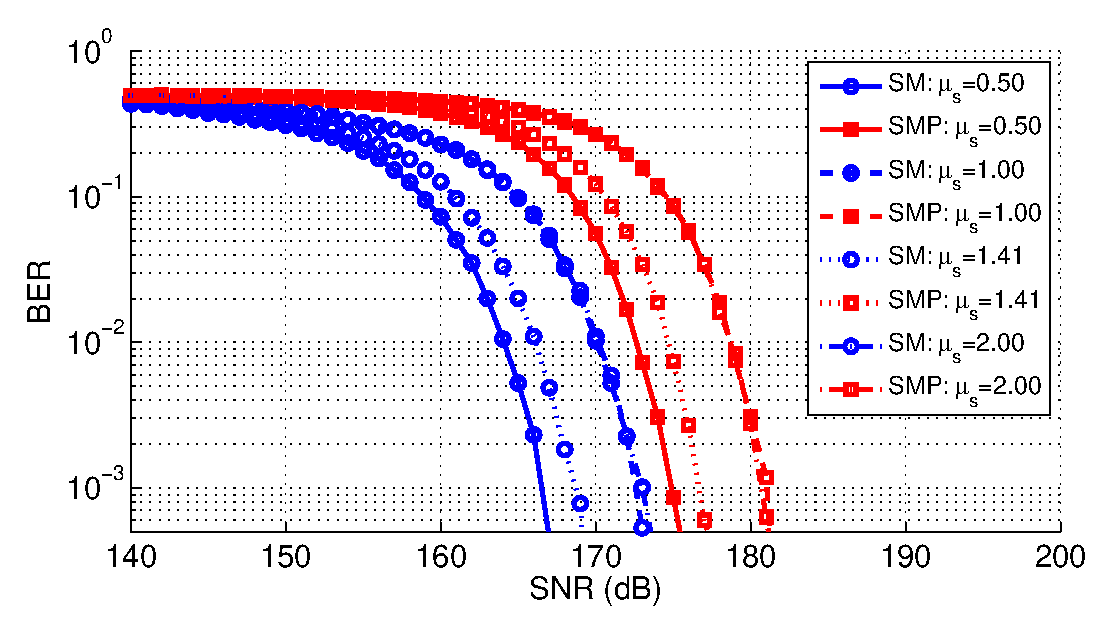
\includegraphics[width=\textwidth]{figMSN4B4.eps}
			\caption{4 bits/sym}
			\label{figMSN4B4}
		\end{subfigure}
		
		\begin{subfigure}{\textwidth}
			\centering
			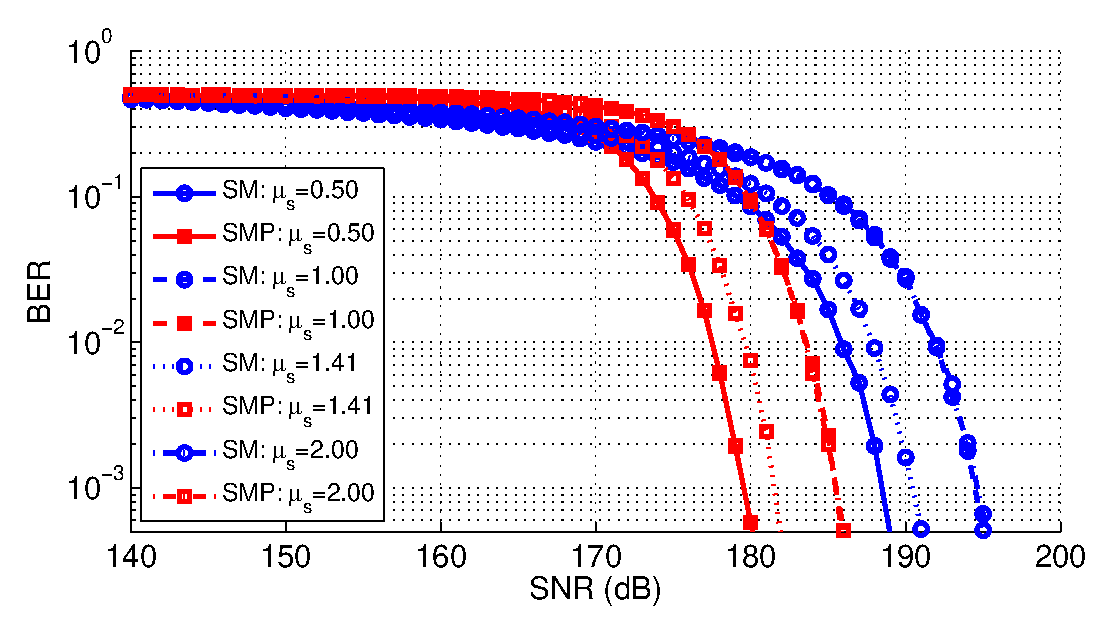
\includegraphics[width=\textwidth]{figMSN4B8.eps}
			\caption{8 bits/sym}
			\label{figMSN4B8}
		\end{subfigure}
		
		\caption{BER vs SNR for different $\mu_{s}$.}
		\label{figMSBvS}
\end{figure}

At lower bit rates, SM benefits from having higher transmit power per symbol at lower M-PAM level. To achieve higher bit-rates, higher M-PAM levels push the constellations closer to each other thus quickly degrading the SM performance as compared to SMP. As shown in \figurename{ \ref{figASBvS}}, \figurename{ \ref{figESBvS}} and \figurename{ \ref{figMSBvS}}, to achieve BER$=10^{-3}$, at 4 bits/sym, SM performs 8-10dB better while at 8 bits/sym, SMP performs 8-10dB better.


%\begin{figure}
	%\centering
		%\begin{subfigure}{\textwidth}
			%\caption{}
			%\label{}
		%\end{subfigure}
		%\caption{}
		%\label{}
%\end{figure}